%%%%%%%%%%%%%%%%%%%%%%%%%%%%%%%%%%%%%%%%%
% University/School Laboratory Report
% LaTeX Template
% Version 3.1 (25/3/14)
%
% This template has been downloaded from:
% http://www.LaTeXTemplates.com
%
% Original author:
% Linux and Unix Users Group at Virginia Tech Wiki 
% (https://vtluug.org/wiki/Example_LaTeX_chem_lab_report)
%
% License:
% CC BY-NC-SA 3.0 (http://creativecommons.org/licenses/by-nc-sa/3.0/)
%
%%%%%%%%%%%%%%%%%%%%%%%%%%%%%%%%%%%%%%%%%

%----------------------------------------------------------------------------------------
%	PACKAGES AND DOCUMENT CONFIGURATIONS
%----------------------------------------------------------------------------------------

\documentclass{article}

\usepackage{siunitx} % Provides the \SI{}{} and \si{} command for typesetting SI units
\usepackage{graphicx} % Required for the inclusion of images
\usepackage[italian]{babel} 
\usepackage[utf8]{inputenc}
\usepackage{natbib} % Required to change bibliography style to APA
\usepackage{amsmath} % Required for some math elements
\usepackage{mathtools}
\usepackage{url}
\usepackage[section]{placeins}
\usepackage{subcaption}
\renewcommand{\refname}{Bibliografia}
\renewcommand{\contentsname}{Indice}
\DeclareSIUnit{\poise}{P}

\setlength\parindent{0pt} % Removes all indentation from paragraphs

\renewcommand{\labelenumi}{\alph{enumi}.} % Make numbering in the enumerate environment by letter rather than number (e.g. section 6)

%\usepackage{times} % Uncomment to use the Times New Roman font

%----------------------------------------------------------------------------------------
%	DOCUMENT INFORMATION
%----------------------------------------------------------------------------------------

\title{\vspace{-2cm} Modellazione della microcircolazione retinica\\tramite analogia fluido - elettrica} % Title

\author{Giulio Gargantini} % Author name

\date{Ottobre 2019} % Date for the report

\begin{document}

\maketitle % Insert the title, author and date

\begin{center}
Prof. A.G. Mauri \\
Computational Models for Electronics and Biomathematics\\
Politecnico di Milano\\
A.A. 2018/2019
\end{center}

% If you wish to include an abstract, uncomment the lines below
\begin{abstract}
In questo progetto si è voluto simulare la microcircolazione nella retina modellandola come un circuito elettrico a resistenze variabili con l'obiettivo di replicare i risultati di \cite{art1}.
L'attenzione è rivolta in particolare alla stima del flusso sanguigno nella microcircolazione per individui aventi valori diversi di pressione sanguigna e pressione intraoculare.
\end{abstract}

\tableofcontents
\newpage
%----------------------------------------------------------------------------------------
%	INTRO
%----------------------------------------------------------------------------------------

\section{Introduzione}
Nello studio della fisiologia dell'apparato visivo e nella ricerca relativa ad alcune sue disfunzioni, una buona comprensione della microcircolazione sanguigna a livello della retina riveste un ruolo fondamentale.
La retina è irrorata da una rete di vasi esposti alla pressione interna del bulbo oculare, la quale può, se alterata, inibire un corretto afflusso di sangue e favorire l'insorgenza di patologie come il glaucoma.
Vista l'importanza cruciale dell'individuazione delle cause precise di una malattia tanto invalidante, i ricercatori si sono concentrati sullo sviluppo di modelli capaci di simulare in modo efficace la microcircolazione retinica e le sue interazioni con la struttura dell'occhio.

Il modello su cui si concentra questo progetto è presentato in \cite{art1} e sfrutta l'analogia elettrico-idraulica (cfr. capitolo 4 di \cite{notes}) per modellare la rete di vasi sanguigni come un circuito elettrico a resistenze variabili.
Ciò permette di prendere in considerazione l'azione della pressione intraoculare (IOP) e della pressione sanguigna sulla larghezza dei vasi, strettamente correlata alla resistenza idraulica degli stessi e al flusso di sangue complessivo in un ciclo cardiaco.

Questo rapporto si articola in quattro parti principali.
Nella prima si illustra il quadro generale del problema partendo dall'anatomia e fisiologia delle porzioni dell'occhio analizzate, per poi procedere, nella seconda parte, alla deduzione di un modello ridotto della microcircolazione secondo l'analogia fluido-elettrica.
Nella terza si illustra l'implementazione del modello ricavato nella sezione precedente tramite un codice Matlab e si presentano le relazioni principali tra le diverse funzioni.
Infine la quarta parte è dedicata ai risultati ottenuti e al confronto con quelli ottenuti in \cite{art1}, discutendone il significato fisico e l'importanza.

%----------------------------------------------------------------------------------------
%	SECTION 1
%----------------------------------------------------------------------------------------

\section{Anatomia e fisiologia}
In questa sezione si descrivono le componenti dell'occhio che vengono studiate nel modello in esame.
\begin{figure}[h]
\begin{center}
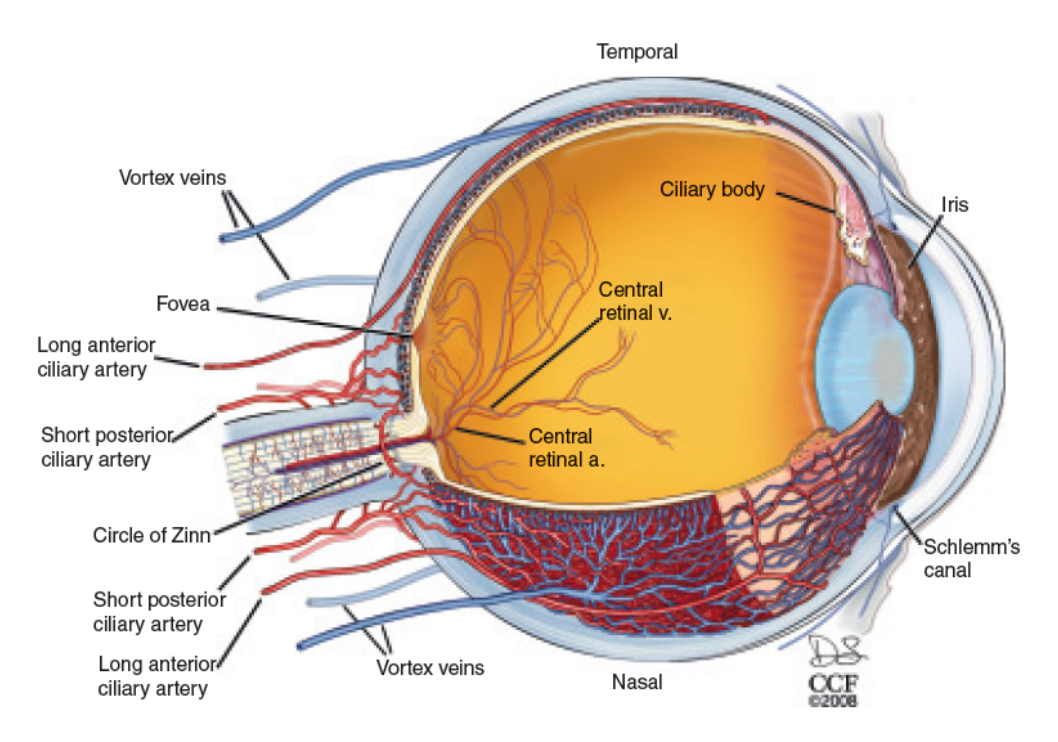
\includegraphics[width=0.8\textwidth]{Pictures/occhio.png}
\caption{Struttura generale dell'occhio \cite{Tesi}}
\label{eyeball}
\end{center}
\end{figure}
L'occhio ha una forma grossomodo sferica, la cui porzione centrale è occupata dall'umore vitreo, una sostanza gelatinosa e trasparente che mantiene la tonicità del globo oculare. 
L'umor vitreo è completamente racchiuso dalla sclera, una membrana di tessuto fibroso di colore bianco, ad eccezione della parte anteriore in cui esso è limitato dal cristallino.
Tra il cristallino e la cornea, la membrana trasparente che separa l'occhio dall'esterno, si trovano due sezioni, dette camera anteriore e posteriore, separate dall'iride e contenenti l'umor acqueo.

Sulla parte posteriore dell'occhio, adagiata sulla sclera, si trova la retina: un tessuto fotosensibile capace di trasformare i segnali luminosi in impulsi nervosi i quali, raccolti dal nervo ottico, vengono inviati al cervello \cite{Tesi}.
\subsection{Anatomia della retina}
A differenza della sclera, irrorata da molteplici vasi sanguigni come le arterie e le vene ciliari e le vene vorticose, gli unici collegamenti tra la rete di capillari della retina e il flusso sanguigno sono l'Arteria Retinica Centrale (CRA) e la Vena Retinica Centrale(CRV).
\begin{figure}[h]
\begin{center}
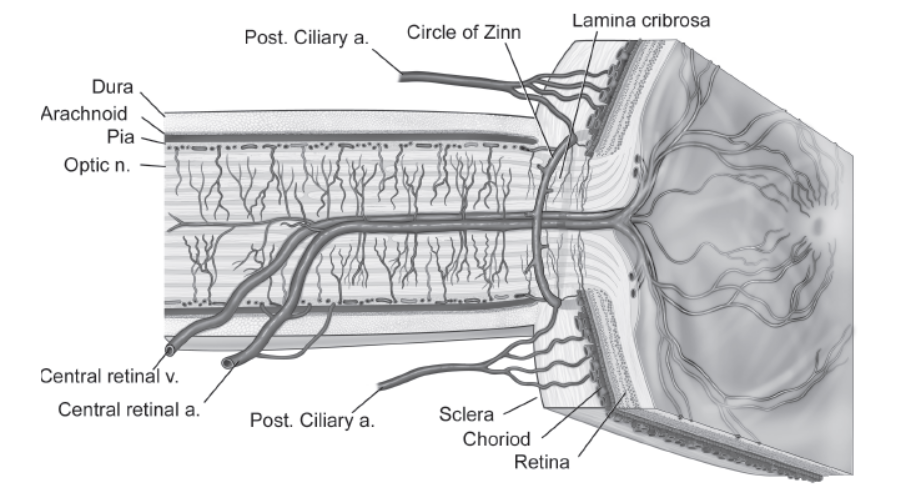
\includegraphics[width=0.8\textwidth]{Pictures/Optic_nerve.png}
\caption{Principali vasi retinici \cite{Tesi}}
\label{retina}
\end{center}
\end{figure}
Entrambi i vasi percorrono un tratto all'interno del nervo ottico, circondati dalle fibre nervose e entrano nell'occhio attraverso la Lamina Cribrosa: tale lamina è una porzione della sclera forata in molteplici punti, attraverso la quale passano le fibre innervanti la retina, la CRA e la CRV (cfr. figura \ref{retina}).
A questo punto l'arteria centrale si divide in molteplici arteriole e capillari, i quali, dopo aver irrorato le cellule della retina, si ricongiungono formando una rete di venule che, a loro volta, si uniscono nella CRV.

I vasi sanguigni non hanno pareti rigide, quindi la loro sezione è soggetta a variazioni dovute alla differenza tra la pressione esterna e interna al vaso: nella zona del nervo ottico i vasi sono soggetti alla pressione del tessuto retrolaminare (RLTp) mentre all'interno del bulbo oculare sono esposti alla pressione intraoculare (IOP).
Vene e arterie sono costituite da tessuti diversi e hanno una diversa struttura: le prime sono generalmente più fini delle seconde e devono sostenere una pressione interna più debole.
Per questo motivo esse sono più soggette ad ampie variazioni di volume e al rischio di collassare su loro stesse se la pressione interna non è in grado di controbilanciare quella agente sulle pareti della vena.
\subsection{Circolazione dell'umor acqueo}
La pressione interna dell'occhio (IOP) è mantenuta grazie alla produzione di umor acqueo.
Questo liquido trasparente simile al plasma è prodotto dal corpo ciliare nella camera posteriore dell'occhio, da cui filtra nella camera anteriore attraverso l'iride e la pupilla.
Dalla camera anteriore esso passa attraverso il trabecolato, una struttura porosa posta tra la sclera e la cornea, per esser drenato nel canale di Schlemm per disperdersi infine nella circolazione venosa (cfr. figura \ref{umoracqueo}).
\begin{figure}[h]
\begin{center}
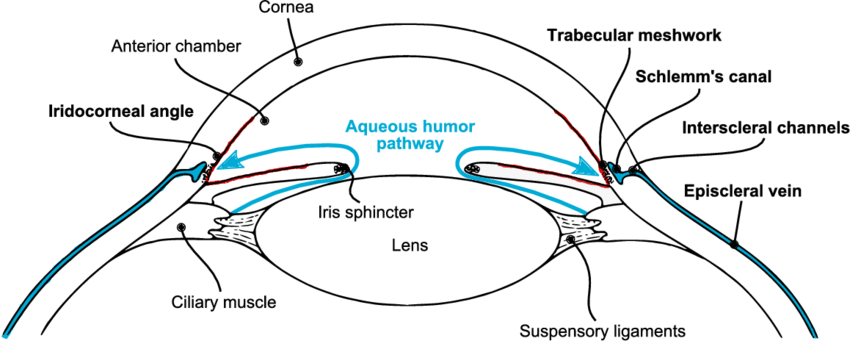
\includegraphics[width=0.8\textwidth]{Pictures/umor_acqueo.png}
\caption{Circolazione dell'umor acqueo nelle camere posteriore e anteriore \cite{Tesimmagine}}
\label{umoracqueo}
\end{center}
\end{figure}
Nel caso in cui non si verifichi un normale drenaggio dell'umor acqueo, ad esempio per l'occlusione del trabecolato, il fluido si accumula nella camera anteriore dell'occhio premendo sul cristallino e trasmettendo la pressione all'umor vitreo, aumentando così l'IOP.
Tale aumento della pressione esterna può provocare il collasso dei vasi sanguigni della retina, in particolare delle vene, diminuendo l'irrorazione  del tessuto e favorendo l'insorgenza del glaucoma.

Per contrastare gli effetti di un'elevata IOP è stata sviluppata la trabeculectomia: un'operazione chirurgica in cui si effettua un foro nella sclera in corrispondenza della camera anteriore, permettendo all'umor acqueo di drenare in una sacca al di sotto  della congiuntiva.
Permettendo nuovamente il drenaggio del fluido si osserva una considerevole riduzione del valore dell'OPP nei pazienti, riportandolo ai livelli fisiologici (cfr. tabela 6 di \cite{art1}).
%----------------------------------------------------------------------------------------
%	SECTION 2
%----------------------------------------------------------------------------------------

\section{Derivazione del modello}
\subsection{Analogia fluido - elettrica}
Nel capitolo 4 di \cite{notes} si presenta in dettaglio l'analogia fluido - elettrica, ovvero come una rete di tubi percorsi da un fluido incomprimibile si possa descrivere con le stesse equazioni cusate per modellare i circuiti elettrici.
Si consideri il flusso come l'analogo della corrente e la pressione del fluido corrispondente al potenziale elettrico in un punto del circuito.
Sotto quest'analogia si osserva che la caduta di pressione ai due capi di un tubo si può interpretare come l'effetto di una resistenza idraulica e le proprietà elastiche di una sezione della rete, che permettono a una porzione del vaso di accumulare il fluido, si possono ricondurre agli effetti capacitivi di un condensatore.
Inoltre si può mostrare che le leggi di Kirchhoff per il potenziale e per la corrente sono ugualmente valide in questo contesto.

Senza ripetere i calcoli che portano a definire l'analogia fluido - elettrica, si riportano nella tabella \ref{tab_analogia} le equivalenze tra le grandezze principali e le unità di misura utilizzate.

\begin{table}[h!]
\begin{center}
\begin{tabular}{| c | c |}
\hline
\textbf{Grandezza elettrica} & \textbf{Grandezza idraulica}\\
\hline
Tensione [\si{\volt}] & Pressione [\si{\mmHg}]\\
Corrente [\si{\ampere}] & Flusso [\si{\milli\liter \per \minute}]\\
Carica [\si{\coulomb}] & Volume [\si{\milli\liter}]\\
Resistenza elettrica [\si{\ohm}] & Resistenza idraulica [\si{\mmHg \second \per \milli\liter}]\\
Capacità elettrica [\si{\farad}] & Capacità idraulica [\si{\milli\liter \per \mmHg}]\\
\hline
\end{tabular}
\caption{Confronto tra grandezze equivalenti nell'analogia fluido - elettrica e corrispondenti unità di misura}
\label{tab_analogia}
\end{center}
\end{table}


\subsection{Deduzione del circuito}
I vasi della microcircolazione retinica si possono dividere in cinque compartimenti: la CRA, le arteriole, i capillari, le venule e la CRV numerati da $1$ a $5$.
Ciascun compartimento può essere diviso in sezioni rappresentanti le diverse porzioni dei vasi e ciascuna di esse è modellata come un resistore in un circuito elettrico.
Ogni resistore è identificato dal numero del compartimento corrispondente e da una lettera.
Essendo le pareti dei vasi sanguigni elastiche, vene e arterie possono variare il loro volume e immagazzinare del sangue nel corso del ciclo cardiaco: tale proprietà è descritta da una capacità assegnata ad ogni compartimento ed è rappresetata nel modello circuitale tramite dei condensatori.

\begin{figure}[h]
\begin{center}
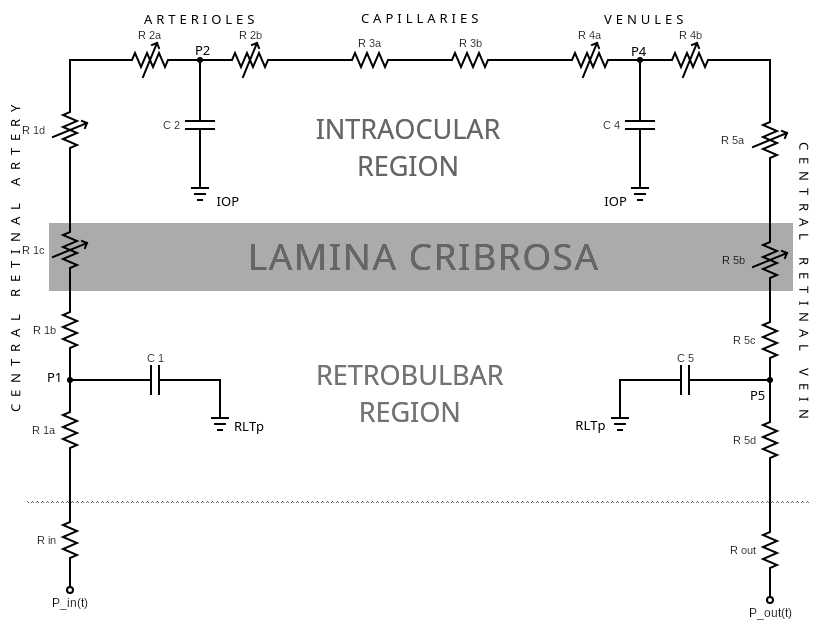
\includegraphics[width=1.0\textwidth]{Pictures/circuit1.png}
\caption{Rappresentazione circuitale della microcircolazione retinica \cite{art1}}
\label{circuito}
\end{center}
\end{figure}

Il modello adottato in \cite{art1} rappresenta la microcircolazione retinica tramite il circuito rappresentato nella figura \ref{circuito}.
La CRA e la CRV sono gli unici vasi che attraversano la lamina cribrosa passando dal nervo ottico alla regione intraoculare.
Per questo motivo tali compartimenti sono rappresentati tramite quattro resistori: due per la regione retrobulbare, uno per la porzione di vaso che attraversa la lamina cribrosa e uno per la regione intraoculare.
Le sezioni dei vasi nella regione retrobulbare sono sottoposte alla pressione del tessuto retrolaminare (RLTp), la porzione all'interno dell'occhio è sottoposta alla pressione intraoculare (IOP) mentre la pressione esercitata dalla lamina cribrosa è modellata seguendo il modello descritto in \cite{art3} e descritta in una sezione dedicata.
La sezione nella regione retrobulbare è divisa in due resistori per ciascun vaso ($R_{1a}$, $R_{1b}$ e $R_{2a}$, $R_{2b}$ rispettivamente) in modo che i corrispondenti condensatori $C_1$ e $C_5$ agiscano sulla pressione media dei vasi nel nervo ottico.

I compartimenti delle arteriole, capillari e venule sono modellati tramite due resistori ciascuno.
Arterie e venule sono modellate tramite i condensatori $C_2$ e $C_4$ connessi in modo tale che le proprietà capacitive agiscano sulle pressioni medie in ciascuno dei compartimenti.
Non essendo i capillari dotati di pareti elastiche, la sezione corrispondente non è connessa ad alcun condensatore.

Le pressioni $P_{in}$ e $P_{out}$ agli estremi del circuito sono funzioni del tempo  ricavate dalla figura 3c di \cite{art1} e rappresentano le pressioni sanguigne arteriosa e venosa rispettivamente a monte e a valle della microcircolazione; la connessione tra le pressioni in input e il circuito è effettuata tramite i resistori $R_{in}$ e $R_{out}$, rappresentanti i tratti di arteria e di vena prima della CRA e dopo la CRV.

Usando la legge di Kirchhoff per le correnti e la definizione di capacità, dal circuito si può ricavare il seguente sistema di equazioni differenziali ordinarie, la cui soluzione permette di ricavare l'evoluzione delle varie grandezze caratteristiche nel tempo e, in ultima analisi, dedurre il comportamento del sistema fisico.

\begin{equation}
\begin{dcases}
  C_1 \frac{d}{dt}(P_1 - RLT_p) &= \frac{P_{in} - P_1}{R_{in} + R_{1a}}  - \frac{P_1 - P_2}{R_{1b} + R_{1c} + R_{1d} + R_{2a}} \\
  C_2 \frac{d}{dt}(P_2 - IOP) &= \frac{P_1 - P_2}{R_{1b} + R_{1c} + R_{1d} + R_{2a}}  - \frac{P_2 - P_4}{R_{2b} + R_{3a} + R_{3b} + R_{4a}} \\
  C_4 \frac{d}{dt}(P_4 - IOP) &= \frac{P_2 - P_4}{R_{2b} + R_{3a} + R_{3b} + R_{4a}}  - \frac{P_4 - P_5}{R_{4b} + R_{5a} + R_{5b} + R_{5c}} \\
  C_5 \frac{d}{dt}(P_1 - RLT_p) &= \frac{P_4 - P_5}{R_{4b} + R_{5a} + R_{5b} + R_{5c}}  - \frac{P_5 - P_{out}}{R_{5d} + R_{out}}
\end{dcases}
\label{sistema}
\end{equation}
\subsection{Valore dei resistori}

In \cite{art1} si possono trovare dei valori standard per i resistori del circuito \ref{circuito} calcolati tramite la legge di Poiseuille per uno stato di controllo.
Un circuito lineare composto da resistori costanti non è in grado di caratterizzare la natura elastica dei vasi sanguigni e la dipendenza del flusso dal loro diametro e quindi non è indicato per simulare il fenomeno di collasso dei vasi sanguigni in caso di IOP elevata che si riscontra nei pazienti affetti da glaucoma.

L'articolo \cite{art1} propone, oltre ai classici resistori costanti, tre tipi di resistori adatti a modellare particolari sezioni della microcircolazione.
Tali categorie sono i \textit{compliant resistors}, adatti a modellare vasi la cui pressione media interna è sempre superiore alla pressione esterna (adatti per le sezioni della CRA nella regione intraoculare e in corrispondenza della lamina cribrosa), gli \textit{Starling resistors} o \textit{collapsible resistors} adatti per le vene e le venule, la cui pressione interna può essere inferiore o superiore alla pressione esterna, e infine gli \textit{active resistors} per modellare le arteriole, le quali possono modificare il proprio diametro a seconda delle circostanze secondo il processo di autoregolazione (cfr. \cite{Tesi}). 
Uno schema che illustra il modello adottato per ciascun resistore del circuito si può trovare alla figura \ref{circuitocolori}.

\begin{figure}[h]
\begin{center}
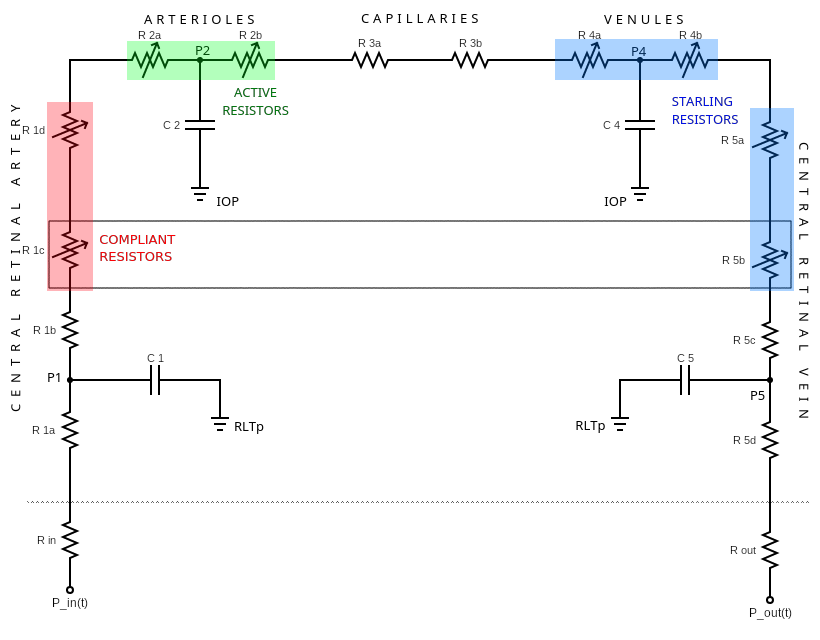
\includegraphics[width=1.0\textwidth]{Pictures/circuit2.png}
\caption{Resistori variabili \cite{art1}}
\label{circuitocolori}
\end{center}
\end{figure}

\subsubsection*{Compliant resistors}
Nel modello in esame, il sangue arterioso nella CRA è sempre a pressione maggiore rispetto alla pressione esterna al vaso; perciò le varie sezioni dell'arteria avranno generalmente un diametro superiore a quello dello stato di riposo e ad un aumento della pressione nel vaso corrisponderà un aumento del suo diametro e una conseguente riduzione della resistenza idraulica.
Tale ipotesi è ragionevole: nella circolazione arteriosa la pressione risente direttamente della pulsazione cardiaca, che viene trasmessa lungo i vasi dalle pareti delle arterie, caratterizzate dalla presenza di fibre muscolari.
Nel modello in esame si prende come valore per la pressione d'ingresso  i $2/3$ del valore della pressione in corrispondenza dell'arteria brachiale per tenere conto della distanza di questa dall'occhio.

Dalla legge di Laplace per un cilindro comprimibile e dalla leggge di Poiseuille (cfr. \cite{art1}, capitolo 4 di \cite{notes} e \cite{Libro}) si ricava la seguente formula per il \textit{compliant resistor},
\begin{equation}
R = \frac{k_r \rho L}{\mathcal{A}_{ref}^2}\left( 1 + \frac{\Delta P}{k_p k_L}\right)^{-4}
\label{compliantR}
\end{equation}
dove $\rho$ è la densità del sangue, $L$ e $\mathcal{A}_{ref}$ rispettivamente la lunghezza e la sezione del vaso a riposo e $\Delta P = P_{int} - P_{ext}$ la differenza di pressione ai due lati della parete.
I termini restanti sono costanti che dipendono dalla viscosità $\mu$, dal modulo di Young $E$, dal coefficiente di Poisson $\nu$ e dallo spessore $h$ della parete secondo le seguenti relazioni: $k_r = 8 \pi \mu / \rho$, $k_p = E h^3 / \sqrt{1 - \nu^2}\  (\pi/\mathcal{A}_{ref})^{3/2}$, $k_L = 12 \mathcal{A}_{ref} / \pi h^2$.
\subsubsection*{Starling resistors}
Il modello adottato per modellare le vene è più complesso: il sangue venoso si trova ad una pressione molto inferiore rispetto a quello arterioso, perciò è possibile che la pressione interna al vaso sanguigno sia inferiore a quella esterna, provocando uno schiacciamento della vena.
Tale deformazione può essere molto accentuata, specialmente visto il sottile spessore delle vene rispetto alle arterie, quindi si possono verificare drastici aumenti della resistenza per tali sezioni di vasi sanguigni.
Un modello efficace per tali sezioni del circuito è presentato nel capitolo 4 di \cite{notes} e distingue due comportamenti per il resistore: se la differenza di pressione tra l'interno e l'esterno è positiva ($\Delta P > 0$), la resistenza si trova utilizzando la formula del \textit{compliant resistor} (\ref{compliantR}), se invece $\Delta P < 0$ si usa una formula alternativa che tiene conto degli effetti della deformazione della membrana.

\begin{equation}
R = \begin{dcases}
\frac{k_r \rho L}{\mathcal{A}_{ref}^2}\left( 1 + \frac{\Delta P}{k_p k_L}\right)^{-4} & \Delta P \ge 0\\
\frac{k_r \rho L}{\mathcal{A}_{ref}^2}\left( 1- \frac{\Delta P}{k_p}\right)^{4/3} & \Delta P < 0\\
\end{dcases}
\label{starlingR}
\end{equation}
I parametri presenti nella definizione sono definiti come per il \textit{compliant resistor}.

La modellazione della sezione 4 richiede un'attenzione particolare: infatti, essa non corrisponde a un vaso specifico, ma a un reticolo di venule aventi diametro, sezione e spessore differente; inoltre le venule sono i vasi più esposti all'azione dell'IOP e quindi sono le più soggette a fenomeni di ipercompressione, che questo progetto si propone di simulare.
Sono stati provati diversi approcci per modellare la struttura complessa della rete di venule; in particolare si segnalano l'approccio gerarchico a due livelli (\textit{small vessels} e \textit{large vessels} adottato in \cite{Libro}), l'approccio mutiscala adottato da \cite{art1} e \cite{Tesi}, dove sono considerati tredici diversi livelli di venule, e l'approccio monolitico in cui la complessità dei vasi è ridotta a un piccolo insieme di parametri mediati (tentativi sono stati fatti con i dati di \cite{art2} e di \cite{Duker}).
Il metodo ritenuto è una semplificazione del'approccio usato in \cite{art1} usando come valore di base della resistenza per $\Delta P = 0$ il valore di controllo per il resistore riportato nell'articolo, e i parametri $k_r$, $k_p$ e $k_L$ non sono esplicitamente calcolati ma dedotti dai rapporti tra le altre grandezze relative alle venule, come il rapporto tra lume e spessore.

\subsubsection*{Active resistors}
Nella figura \ref{circuitocolori} si può osservare come per le arteriole non si sia adottato lo stesso modello usato per la CRA.
Infatti esse sono soggette a un fenomeno di autoregolazione che permette una variazione di volume in risposta a stimoli come la pressione esterna, o la concentrazione di diossido di carbonio.
Tale meccanismo varia da individuo a individo e talvolta è completamente assente e uno degli obiettivi del progetto è verificarne l'incidenza sul'irrorazione della retina.
Una trattazione dettagliata dell'autoregolazione nella microcircolazione arteriosa si può trovare in \cite{Tesi}, ma per questo progetto ci si è limitati a un modello semplificato proposto in \cite{art1} che fa dipendere il valore della resistenza delle arteriole $R_{2a}$ e $R_{2b}$ solo dalla pressione di perfusione oculare (OPP) definita come $OPP = 2/3 MAP - IOP$, dove $MAP$ è la pressione arteriosa media.
Secondo questo modello le resistenze $R_{2a}$ E $R_{2b}$ hanno lo stesso valore e, per individui aventi un meccanismo di autoregulazione funzionale, lo si può calcolare usando la seguente formula.

\begin{equation}
R = \bar{R}_{2a} \frac{c_L + c_U \exp \left[ K \left(Q_{noAR}(OPP) - \bar{Q}\right) - \hat{c}\right]}{1 + \exp \left[ K \left(Q_{noAR}(OPP) - \bar{Q}\right) - \hat{c}\right]}
\label{activeR}
\end{equation}

In questo caso $c_L$ e $c_U$ sono i valori minimo e massimo della resistenza, $K$ è la sensitività della resistenza a variazioni di pressione e $\hat{c}$ è una costante di normalizzazione.
$\bar{R}_{2a}$ è il valore di controllo per una delle resistenze delle arteriole e corrisponde al valore adottato in assenza di autoregolazione funzionale.
$\bar{Q}$ rappresenta il flusso medio in stato di controllo e $Q_{noAR}(OPP)$ è il flusso che si avrebbe in caso di autoregolazione assente per un OPP assegnato.
Operativamente, i valori assunti da $Q_{noAR}(OPP)$ sono stati estratti dalla figura A2 destra di \cite{art1}.

\begin{figure}[h]
\begin{center}
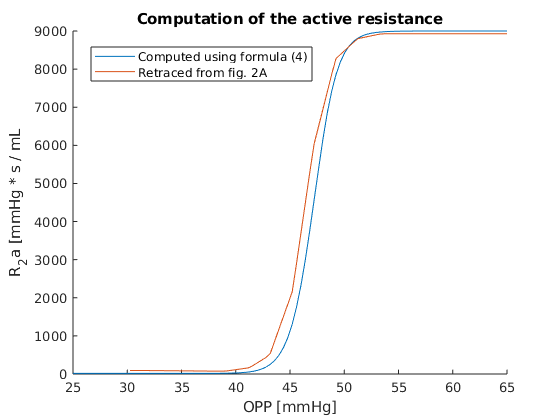
\includegraphics[width=1.0\textwidth]{Pictures/compare_R2a.png}
\caption{Confronto tra i risultati della formula (4) di \cite{art1} e il grafico in figura 2A sinistra dello stesso articolo}
\label{compare_active}
\end{center}
\end{figure}

\subsection{Pressione nella Lamina Cribrosa}
\label{sez_lamcri}
Come accennato nella sezione precedente, pre passare dalla regione retrobulbare a quella intraoculare, le fibre del nervo ottico e l'arteria e la vena retiniche centrali devono attraversare una porzione porosa della sclera detta lamina cribrosa che comprime i vasi esercitando una pressione.
In \cite{art3} si modella la lamina cribrosa come un disco elastico non lineare soggetto all'IOP e all'RLTp sulle sue facce e alla tensione della sclera sul bordo (si veda fig. \ref{laminacribrosa}).

\begin{figure}[h]
\begin{center}
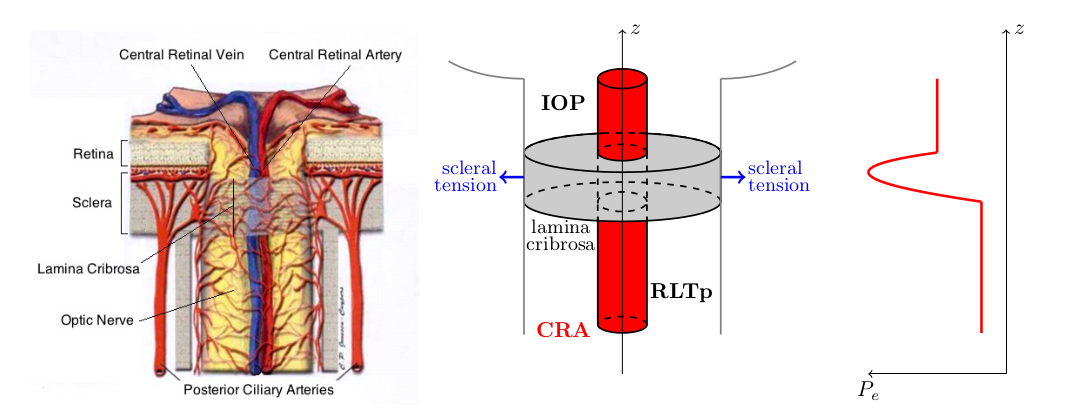
\includegraphics[width=1.0\textwidth]{Pictures/laminacribrosa.png}
\caption{1.Anatomia della lamina cribrosa, 2.Modellazione tramite disco elastico soggetto all'IOP, RLTp e alla tensione sclerale, 3.Andamento della pressione lungo l'asse del nervo ottico \cite{art3}}
\label{laminacribrosa}
\end{center}
\end{figure}

Secondo tale modello si può trovare il valore della pressione esercitato dalla lamina cribrosa sulla CRA, che si suppone passare per il suo centro, calcolando il tensore degli sforzi $\mathbf{S}$ e valutandone la componente $\mathbf{S}_{ss} = u_s \cdot \mathbf{S} u_s$ in $s = 0$, dove $s$ è la coordinata radiale e $u_s$ il vettore unitario associato.
La pressione agente sulle pareti della CRA in ogni punto si ricava quindi tramite la formula

\begin{equation}
P_e(z) = \begin{dcases}
RLTp & \mbox{  se  }  z < z_{lc,c}\\ 
-S_{ss}(0,z) & \mbox{  se  }  z_{lc,c} < z < z_{lc}\\ 
IOP & \mbox{  se  }  z > z_{lc,c}
\end{dcases}
\label{cribrosa_alt}
\end{equation}
dove $z$ è la coordinata assiale, $z_{lc}$ è lo spessore della lamina cribrosa e $z_{lc,c} = \min\left\lbrace z \in (0,z_{lc} \mbox{tc} -S_{ss}(0,z) \geq RLTp\right\rbrace$.

I risultati trovati in \cite{art3} risolvendo numericamente il problema sono riportati nella figura \ref{riscribrosa}.

\begin{figure}[h]
\begin{center}
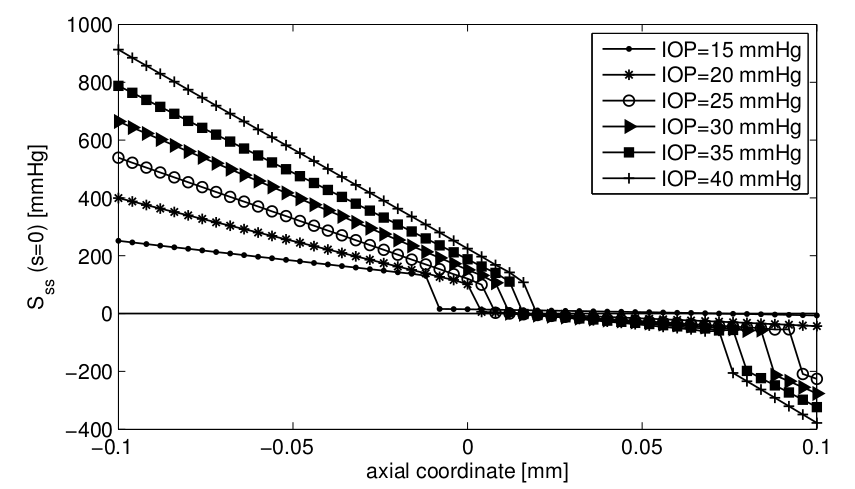
\includegraphics[width=1.0\textwidth]{Pictures/riscribrosa.png}
\caption{Risultati dell'integrazione numerica del tensore degli sforzi della lamina cribrosa in \cite{art3}. Si osservi come l'andamento di $-S_{ss}$ lungo la coordinata assiale sia non lineare e come esso dipenda dall'IOP.}
\label{riscribrosa}
\end{center}
\end{figure}

Tale modello non è compatibile con quello del \textit{compliant resistor} presentato in precedenza, in quanto quello prevede una pressione esterna e interna costanti lungo l'asse del vaso sanguigno.
Nell'implementazione numerica si è utilizzato come pressione agente sul resistore $R_{3c}$, che corrisponde alla porzione della CRA passante per la lamina cribrosa, la media integrale della funzione (\ref{cribrosa_alt}) lungo l'asse della lamina, ottenuta interpolando i punti della figura \ref{riscribrosa} per l'opportuno valore d'IOP.

%----------------------------------------------------------------------------------------
%	SECTION 3
%----------------------------------------------------------------------------------------
\section{Implementazione numerica}
In questa sezione è discussa l'implementazione del modello presentato nella sezione precedente: in particolare nella prima parte si descrive la struttura del codice Matlab usato per la simulazione, mentre nella seconda si presentano i dati utilizzati.
\subsection{Struttura del codice}
I metodi Matlab implementati per la simulazione del modello di microcircolazione si possono dividere in quattro gruppi: le funzioni direttamente chiamate dal main, le funzioni di supporto all'inizializzazione dei dati, quelle chiamate all'interno di \texttt{ode15s} per il calcolo della derivata temporale e quelle necessarie per l'update dei resistori variabili.
\subsubsection*{Funzioni del main}
Sono stati scritti due diversi main per simulare aspetti diversi del modello.
Il \texttt{main1.m} permette di plottare, fissati l'OPP, la pressione arteriosa (bassa, media o alta) e la presenza o meno del meccanismo di autoregolazione delle arteriole, l'evoluzione delle pressioni nei quattro nodi $P_1$, $P_2$, $P_4$ e $P_5$ segnati in figura \ref{circuito},il valore dei vari resistori variabili nel tempo e la velocità e il flusso sanguigno nella CRA e nella CRV, oltre che a calcolare il valore totale del flusso di sangue passante per la CRA nel corso di una pulsazione cardiaca.
Il secondo, \texttt{main2.m} permette di calcolare il valore del flusso complessivo attraverso la CRA nel corso di una pulsazione per un ampio range di valori di OPP, simulando i casi di pazienti con diverse pressioni arteriose e con meccanismo di autoregolazione regolare o disfunzionante.

Nonostante ciò, \texttt{main1.m} e \texttt{main2.m} presentano una struttura molto simile e chiamano le stesse funzioni nello stesso ordine, quindi è possibile descriverli in un'unica sezione.
Entrambi i file cominciano con l'introduzione delle variabili globali \texttt{resistors} e \texttt{data}: la prima raccoglie la serie temporale dei valori assunti dai resistori variabili nel tempo e il valore dei flussi sanguigni nella CRA e nella CRV, la seconda riunisce tutti i parametri del problema ed è inizializzata tramite la funzione \texttt{define\char`_constants}, che sarà discussa in dettaglio più avanti.
È necessario che tali variabili siano globali in quanto devono essere accessibili da tutte le altre funzioni del codice, specialmente dalle funzioni attivate da una chiamata attraverso \texttt{ode15s}.
Dopo l'inizializzazione, si chiama la funzione \texttt{solve\_circuit\_1245} per ottenere una guess iniziale per il vettore $P_{1245} = [P_1, P_2, P_4, P_5]^T$: per farlo, la funzione \texttt{solve\_circuit\_1245} risolve il circuito elettrico avente le resistenze di controllo costanti al posto dei resistori variabili applicando le leggi di Kirchhoff.

Una volta trovata una guess iniziale e definita la durata della pulsazione cardiaca, si usa il solutore \texttt{ode15s} per risolvere il sistema d'ODE (\ref{sistema}) tramite la chiamata \texttt{[ttout, PP1245] = ode15s(\@time\_deriv\_P1245, tspan, P1245,opt)}.

La funzione \texttt{\@time\_deriv\_P1245}, dato un istante di tempo e una situazione iniziale, calcola la derivata temporale del sistema in quel momento.
Una volta integrato il sistema (\ref{sistema}) lungo la durata di una pulsazione, la variabile \texttt{PP1245} contiene l'evoluzione nel tempo di $P_1$, $P_2$, $P_4$ e $P_5$, mentre la struct \texttt{resistors} contiene il valore delle resistenze variabili e del flusso attraverso la CRA e la CRV per ogni istante di tempo.
In \texttt{main1.m}, Dopo una fase di postprocessing, tali valori sono plottati ed è calcolato il valore del flusso totale.

In \texttt{main2.m} l'intera procedura è ripetuta diverse volte per pazienti aventi bassa, media o alta pressione sanguigna e meccanismo di autoregolazione funzionante o alterato e per diversi valori di OPP
I plot delle pressioni non vengono effettuati, ma si registra nella variabile \texttt{Qs} il valore del flusso in funzione dell'OPP per ciascuna delle sei classi di paziente.
Infine, tali valori sono plottati in un unico grafico che permette di confrontare la dipendenza del flusso sanguigno dalla pressione intraoculare per diversi pazienti.

\begin{figure}[h]
\begin{center}
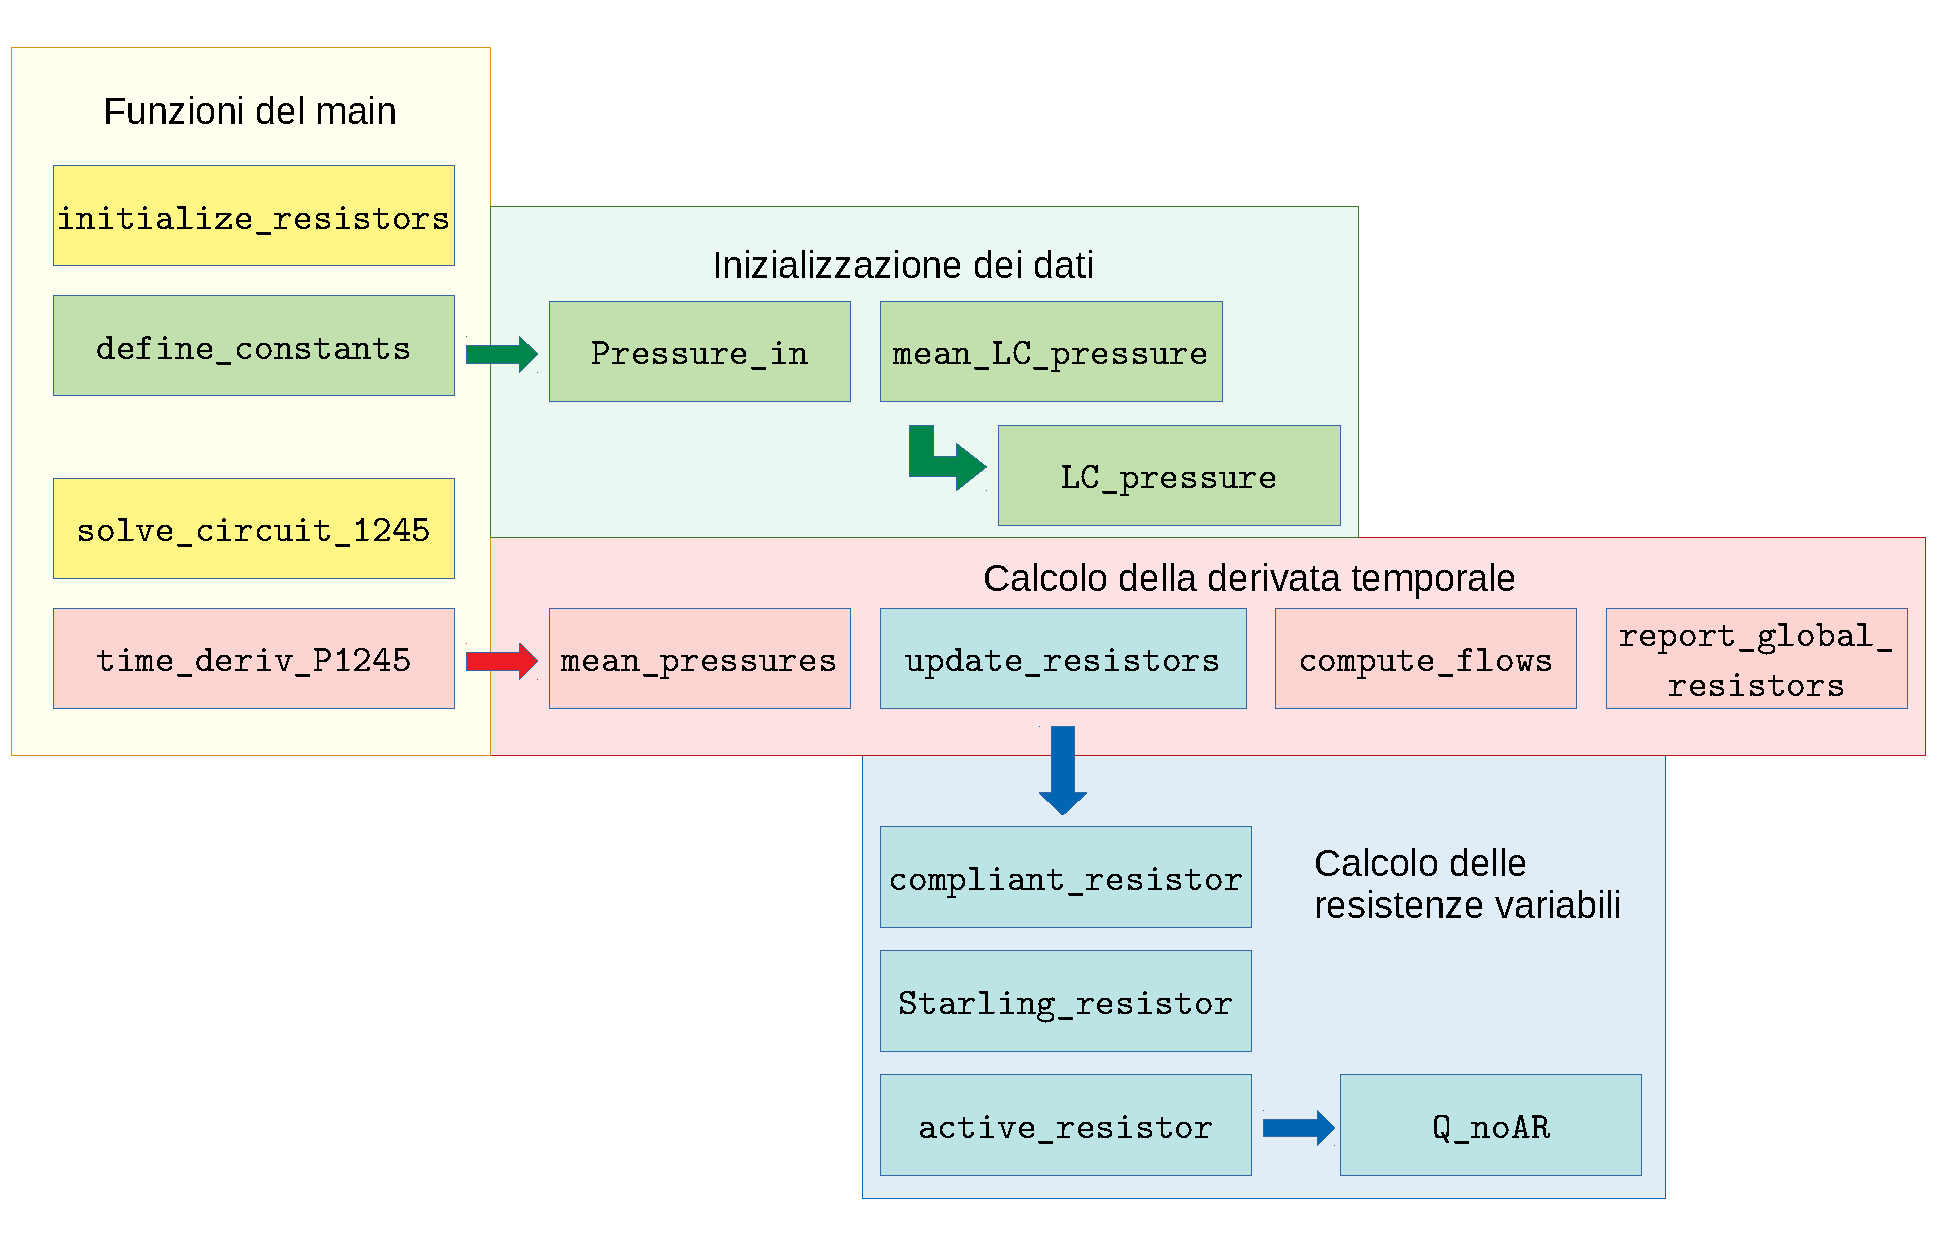
\includegraphics[width=1.0\textwidth]{Pictures/class_diagram.pdf}
\caption{Diagramma delle principali funzioni usate nella simulazione}
\label{diagramma_classi}
\end{center}
\end{figure}
\subsubsection*{Inizializzazione dei dati}

Per entrambi i main, una delle prime operazioni da effettuare è l'inizializzazione della variabile globale di tipo struct \texttt{data} con i dati del problema.
Per farlo, si utilizza la funzione \texttt{define\_constants} che può avere uno, due o tre parametri in input: il primo è sempre la variabile in cui si vogliono immagazzinare i dati del problema (qui la variabile globale \texttt{data}), il secondo e il terzo sono facoltativi e permettono di configurare i dati del problema per un valore di IOP dato e per definire lo stato della pressione e del sistema di autoregolazione del paziente.

In primo luogo la funzione \texttt{define\_constants} definisce i parametri generali del paziente, per poi procedere all'inizializzazione dei valori della pressione usati dal programma (IOP, RLTp, pressioni diastolica e sistolica, pressioni all'ingresso e all'uscita del circuito) ad eccezione della pressione nella lamina cribrosa, che è inizializzata a parte in una sezione successiva.
Per la definizione della pressione in ingresso si utilizza la funzione \texttt{Pressure\_in} che interpola i dati estratti dalla figura 3 di \cite{art1}.
In seguito sono inizializzati i valori di controllo per le resistenze e per le capacità usati nella simulazione, per poi procedere con la definizione delle costanti caratteristiche della CRA, CRV, arteriole e venule, usate per il calcolo delle resistenze nelle sezioni variabili.

Si procede con il calcolo della pressione nella lamina cribrosa secondo il modello descritto nella sezione \ref{sez_lamcri}: l'interpolazione dei dati della figura \ref{riscribrosa} è effettuata dalla funzione \texttt{LC\_pressure}, mentre \texttt{mean\_LC\_pressure} si occupa di valutare la funzione (\ref{cribrosa_alt}) e integrarla lungo l'asse della lamina per fornire un valore medio della pressione esercitato dalla lamina cribrosa sui vasi sanguigni.
\texttt{define\_constants} termina con la definizione di alcuni fattori di conversione tra unità di misura e con la definizione dei criteri d'arresto per il ciclo while in \texttt{time\_deriv\_P1245}.

\subsubsection*{Calcolo della derivata temporale}
L'integrazione del sistema (\ref{sistema}) si effettua nel main tramite il comando \texttt{[ttout, PP1245] = ode15s(\@time\_deriv\_P1245, tspan, P1245,opt)}, dove \texttt{tspan} è l'intervallo di integrazione, \texttt{P1245} la condizione iniziale, \texttt{opt} le opzioni di integrazione (come il livello di accuratezza) e \texttt{time\_deriv\_P1245} la funzione responsabile del calcolo della derivata temporale di $P_{1245}$ in ogni istante di tempo e per ogni valore di $P_{1245}$.

Nella funzione \texttt{time\_deriv\_P1245} sono in primo luogo importate le variabili globali \texttt{data} e \texttt{resistors}, rispettivamente utilizzate e aggiornate dalla funzione.
Subito dopo si dichiara la variabile permanente \texttt{res}, contenente l'ultimo valore calcolato per i resistori variabili.

Successivamente si esegue un ciclo while in cui ad ogni iterazione si calcolano le pressioni medie nei resistori variabili tramite \texttt{mean\_pressures} e li si aggiornano con la funzione \texttt{update\_resistors} al fine di ricostruire il valore dei resistori che genera una distribuzione delle pressioni conforme all'input.
Il ciclo while termina se due iterazioni successive danno valori per le resistenze simili a meno di una tolleranza definita in \texttt{data} o se le resistenze superano una certa soglia, indicando una mancata convergenza del ciclo e seguita da un messaggio di errore.

Al termine del ciclo while si ha quindi nella variabile \texttt{res} un valore per i resistori variabili che genera la distribuzione di pressione attesa $P_{1245}$.
La funzione procede quindi con il calcolo dei flussi attraverso la CRA e la CRV.
I valori ottenuti per i resistori variabili e per i flussi sanguigni sono registrati nella variabile globale \texttt{resistors}, in modo che essi siano accessibili dal main.
La funzione \texttt{time\_deriv\_P1245} termina con il calcolo della derivata temporale di $P_{1245}$ secondo il sistema (\ref{sistema}).

\subsubsection*{Calcolo delle resistenze variabili}
Il ciclo while di \texttt{time\_deriv\_P1245} ha lo scopo di trovare il valore delle resistenze variabili che producono le distribuzione delle pressioni desiderata nei nodi $P_1$, $P_2$, $P_4$ e $P_5$: per farlo, ad ogni iterazione calcola le pressioni medie in ogni resistore variabile e aggiorna i valori delle resistenze tramite \texttt{update\_resistors} fino a convergenza.

La funzione \texttt{update\_resistors} prende come input le variabili \texttt{data}, contenente i parametri del modello, \texttt{mp}, contenente le pressioni medie nei resistori variabili, e \texttt{res}, la variabile da aggiornare con i valori delle resistenze.
La funzione chiama i metodi opportuni per aggiornare i valori delle resistenze secondo la loro natura, come descritto in figura \ref{circuitocolori}: \texttt{compliant\_resistor} per $R_{1c}$ e $R_{1d}$, \texttt{starling\_resistor} per $R_{4a}$, $R_{4b}$, $R_{5a}$ e $R_{5b}$ e \texttt{active\_resistor} per $R_2a$ e $R2b$, che implementano rispettivamente le equazioni (\ref{compliantR}), (\ref{starlingR}) e (\ref{activeR}).
Per il calcolo dei resistori attivi è chiamata anche la funzione \texttt{Q\_noAR} che permette di calcolare il valore di flusso attraverso $R_{2a}$ in caso di autoregolazione assente interpolando i valori della figura A2.b di \citep{art1}.
Come si vede dalla formula (\ref{activeR}), il valore $Q_{noAR}(OPP)$ è necessario per valutare il valore di $R_{2a}$ e $R_{2b}$ in caso di autoregolazione attiva.

\subsection{Dati utilizzati}
Si riportano in questa sezione i dati utilizzati nell'implementazione Matlab del modello.
Tali valori sono stati presi dall'articolo \citep{art1}, fatta eccezione per i parametri riguardanti la lamina cribrosa, che si possono trovare in \cite{art3}.
Tutti i dati provenienti da grafici sono stati analizzati e convertiti in valori numerici tramite il sito \url{http://www.graphreader.com/} \cite{ricalca}.

\subsubsection*{Parametri fisiologici}
Nelle simulazioni si distinguono tre casi in funzione della pressione sanguigna: pazienti con pressione alta, pressione media e pressione bassa.
Per ciascuno dei tre casi sono dati i valori della pressione sistolica e diastolica, misurati in millimetri di mercurio
\begin{table}[h!]
\begin{center}
\begin{tabular}{| c | c | c |}
\hline
 - & \textbf{Pressione sistolica (SP)} & \textbf{Pressione diastolica (DP)}\\
\hline
\textbf{Pressione alta} & $140\ \si{\mmHg}$ & $90\ \si{\mmHg}$\\
\textbf{Pressione media} & $120\ \si{\mmHg}$ & $80\ \si{\mmHg}$\\
\textbf{Pressione bassa} & $100\ \si{\mmHg}$ & $70\ \si{\mmHg}$\\
\hline
\end{tabular}
\caption{Valori della pressione sanguigna}
\label{tab_pressione}
\end{center}
\end{table}

I valori di $P_{in}$ e di $P_{out}$ sono importati dalla figura 3c di \cite{art1} e riscalati a seconda della pressione sanguigna secondo i rapporti $\max(P_{in}) / SP = 0.7683$ e $\min(P_{in}) / DP = 0.4945$.

La pressione nel tessuto retrolaminare è fissata a $RLTp = 7 \si{\mmHg}$ mentre la pressione intraoculare in \texttt{main1} è fissata a $IOP = 15 \si{\mmHg}$ per individui sani o sottopostisi a trabeculectomia, mentre è posta a $30 \si{\mmHg}$ per pazienti con IOP anormale.
In \texttt{main2} l'IOP è fatto variare uniformemente nell'intervallo $15 \si{\mmHg} - 50 \si{\mmHg}$.

\subsubsection*{Capacità e resistenze}
Nell'articolo \cite{Tesi} i valori di controllo per le capacità e le resistenze delle diverse sezioni della microcircolazione sono stati calcolati a partire dai risultati clinici usando la definizione di capacità e la legge di Poiseuille.
\begin{center}
\begin{equation}
\begin{split}
Q &= C \ \Delta V \\
R &= 128 \mu\ L / \pi D^2
\end{split}
\label{eqcapacity}
\end{equation}
\end{center}
dove $Q$ è il flusso passante per il vaso, $\Delta V$ la sua variazione di volume, $\mu$ la viscosità del sangue (diversa per sangue arterioso e venoso), $L$ la lunghezza della sezione del vaso e $D$ il suo diametro.
I risultati sono i seguenti:

\begin{table}[h!]
\begin{center}
\begin{tabular}{| c | c |}
\hline
\textbf{Compartimento} & \textbf{Capacità}\\
\hline
CRA & $ \SI{7.22e-7}{\milli \liter \per \mmHg}$ \\
Arteriole & $ \SI{7.53e-7}{\milli \liter \per \mmHg}$ \\
Venule & $\SI{1.67e-5}{\milli \liter \per \mmHg}$ \\
CRV & $\SI{1.07e-5}{\milli \liter \per \mmHg}$ \\
\hline
\end{tabular}
\caption{Valori di riferimento per le capacità}
\label{tab_capacita}
\end{center}
\end{table}

\begin{table}[h!]
\begin{center}
\begin{tabular}{| c | c || c | c |}
\hline
- & \textbf{Resistenza idraulica} & - & \textbf{Resistenza idraulica}\\
\hline
$R_{in}$ & $\SI{2.25e4}{\mmHg \sec \per \milli \liter}$ & $R_{3b}$ & $ \SI{5.68e3}{\mmHg \sec \per \milli \liter}$ \\
$R_{1a}$ & $\SI{4.30e3}{\mmHg \sec \per \milli \liter}$ & $R_{4a}$ & $ \SI{3.11e3}{\mmHg \sec \per \milli \liter}$ \\
$R_{1b}$ & $ \SI{4.30e3}{\mmHg \sec \per \milli \liter}$ & $R_{4b}$ & $ \SI{3.11e3}{\mmHg \sec \per \milli \liter}$ \\
$R_{1c}$ & $ \SI{1.96e2}{\mmHg \sec \per \milli \liter}$ & $R_{5a}$ & $ \SI{3.08e2}{\mmHg \sec \per \milli \liter}$ \\
$R_{1d}$ & $ \SI{9.78e2}{\mmHg \sec \per \milli \liter}$ & $R_{5b}$ & $ \SI{6.15e1}{\mmHg \sec \per \milli \liter}$ \\
$R_{2a}$ & $ \SI{6.00e3}{\mmHg \sec \per \milli \liter}$ & $R_{5c}$ & $ \SI{1.35e3}{\mmHg \sec \per \milli \liter}$ \\
$R_{2b}$ & $ \SI{6.00e3}{\mmHg \sec \per \milli \liter}$ & $R_{5d}$ & $ \SI{1.35e3}{\mmHg \sec \per \milli \liter}$ \\
$R_{3a}$ & $ \SI{5.68e3}{\mmHg \sec \per \milli \liter}$ & $R_{out}$ & $ \SI{5.74e3}{\mmHg \sec \per \milli \liter}$ \\
\hline
\end{tabular}
\caption{Valori di riferimento per le resistenze}
\label{tab_resistori}
\end{center}
\end{table}

\subsubsection*{Parametri dei vasi}
Per determinare la resistenza dei settori deformabili della CRA e della CRV si sono usati i parametri descritti nella tabella \ref{tab_CR}.
\begin{table}[h!]
\begin{center}
\begin{tabular}{| l | c | c |}
\hline
\textbf{Grandezza} & \textbf{CRA} & \textbf{CRV}\\
\hline
Diametro $D$& $\SI{175e-3}{\milli \meter}$ &  $\SI{238e-3}{\milli \meter}$\\
Lunghezza totale $L$ & $\SI{10}{\milli \meter}$ &  $\SI{10}{\milli \meter}$\\
--nella zona retrobulbare & $8.8 \SI{8.8}{\milli \meter}$ & $8.8 \SI{8.8}{\milli \meter}$\\
--nella lamina cribrosa  & $\SI{0.2}{\milli \meter}$ & $\SI{0.2}{\milli \meter}$\\
--nella zona intraoculare  & $1.0\SI{1.0}{\milli \meter}$ & $1.0\SI{1.0}{\milli \meter}$\\
Viscosità del sangue $\mu$ & $\SI{3.00}{\centi \poise}$ & $\SI{3.24}{\centi \poise}$\\
Modulo di Young $E$ & $\SI{0.3}{\mega\pascal}$ & $\SI{0.6}{\mega\pascal}$\\
Coefficiente di Poisson $\nu$ & $0.49$ & $0.49$\\
Spessore delle pareti $h$ & $\SI{39.7e-3}{\milli\meter}$ & $\SI{10.7e-3}{\milli\meter}$\\
\hline
\end{tabular}
\caption{Valori di riferimento per CRA e CRV}
\label{tab_CR}
\end{center}
\end{table}

Per le arteriole e le venule i parametri usati sono nelle tabelle \ref{tab_art} e \ref{tab_ven} rispettivamente e sono usati per implementare i modelli di \textit{active resistor} e \textit{Starling resistor}.

\begin{table}[h!]
\begin{center}
\begin{tabular}{| c | c |}
\hline
\textbf{Grandezza} & \textbf{Arteriole}\\
\hline
Resistenza di controllo $\bar{R}_{2a}$ & $ \SI{6.00e3}{\mmHg \sec \per \milli \liter}$ \\
Limite inferiore per la variazione $c_L$ & $\SI{2.50e-3}{}$\\
Limite superiore per la variazione $c_U$ & $1.5$\\
Sensitività $K$ & $\SI{6.91e4}{\second \per \milli \liter}$\\
Flusso di controllo $\bar{Q}$ & $\SI{6.8178e-4}{\milli \liter \per \second}$\\
\hline
\end{tabular}
\caption{Valori di riferimento per le arteriole}
\label{tab_art}
\end{center}
\end{table}


\begin{table}[h!]
\begin{center}
\begin{tabular}{| c | c |}
\hline
\textbf{Grandezza} & \textbf{Venule}\\
\hline
Resistenza di controllo $\bar{R}_{4a}$ & $ \SI{3.11e3}{\mmHg \sec \per \milli \liter}$ \\
Rapporto lume pareti $\alpha$ & $0.05$\\
Modulo di Young $E$ & $\SI{0.66}{\mega\pascal}$\\
Coefficiente di Poisson $\nu$ & $0.49$\\
\hline
\end{tabular}
\caption{Valori di riferimento per le venule}
\label{tab_ven}
\end{center}
\end{table}


%----------------------------------------------------------------------------------------
%	SECTION 4
%----------------------------------------------------------------------------------------
\section{Risultati}
I risultati delle simulazioni effettuate mostrano lo stesso andamento dei grafici in \cite{art1}.
In particolare sono riportati nella prima sezione gli andamenti delle pressioni nei nodi $P_1$, $P_2$, $P_4$ e $P_5$ e delle resistenze variabili nel corso di una pulsazione sanguigna, per poi passare al confronto del flusso sanguigno complessivo in funzione dell'IOP per pazienti con diverse pressioni sanguigne e funzionalità nell'autoregolazione.

\subsection{Pressioni e resistenze nel tempo}
Tramite \texttt{main1.m} siamo in grado di simulare l'andamento delle pressioni nei nodi e delle resistenze variabili nel tempo: di seguito si riportano i risultati per due soggetti con autoregolazione funzionale, pressione arteriosa nella norma ($\SI{80}{\mmHg}$ - $\SI{120}{\mmHg}$) aventi un'IOP di $\SI{15}{\mmHg}$, considerato regolare, e di $\SI{30}{\mmHg}$, considerato anomalo.

\begin{figure}[ht]
\begin{subfigure}{.5\textwidth}
  \centering
  % include first image
  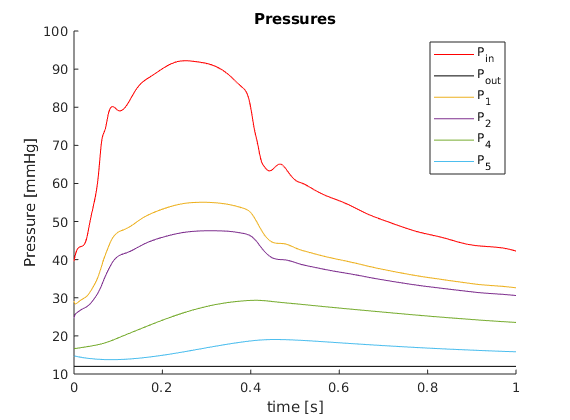
\includegraphics[width=1.0\linewidth]{Pictures/IOP30_part1/pressures_30.png}
\end{subfigure}
\begin{subfigure}{.5\textwidth}
  \centering
  % include second image
  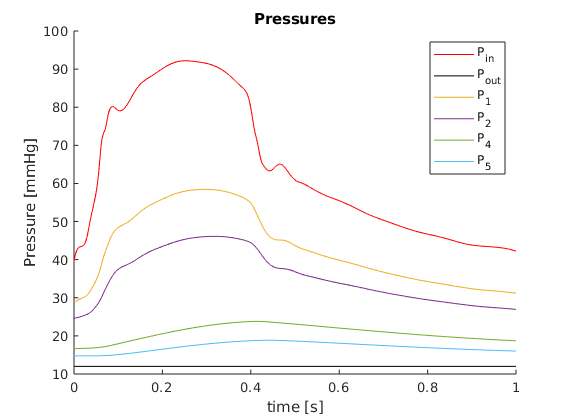
\includegraphics[width=1.0\linewidth]{Pictures/IOP15_part1/pressures_15.png}
\end{subfigure}
\caption{Evoluzione del valore della pressione nei nodi  $P_1$, $P_2$, $P_4$ e $P_5$ per pazienti con $IOP = \SI{30}{\mmHg}$ a sinistra e $IOP = \SI{15}{\mmHg}$ a destra}
\label{pressioni1530}
\end{figure}

\begin{figure}[ht]
\begin{subfigure}{.5\textwidth}
  \centering
  % include first image
  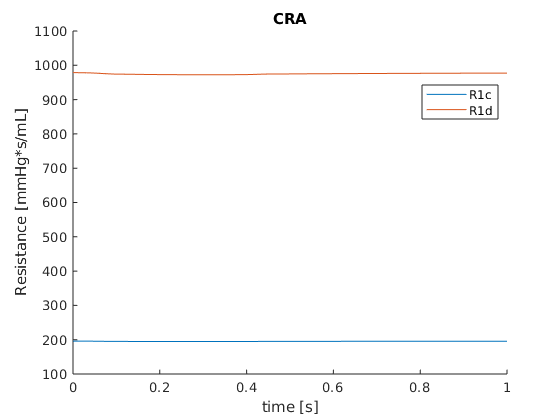
\includegraphics[width=1.0\linewidth]{Pictures/IOP30_part1/CRA_30.png}
\end{subfigure}
\begin{subfigure}{.5\textwidth}
  \centering
  % include second image
  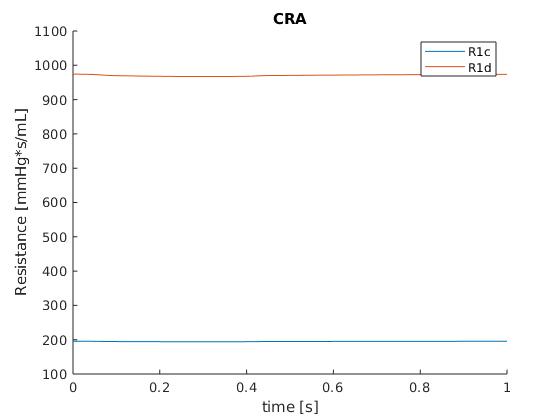
\includegraphics[width=1.0\linewidth]{Pictures/IOP15_part1/CRA_15.png}
\end{subfigure}
\caption{Evoluzione della resistenza nella CRA per pazienti con $IOP = \SI{30}{\mmHg}$ a sinistra e $IOP = \SI{15}{\mmHg}$ a destra}
\label{CRA1530}
\end{figure}

\begin{figure}[ht]
\begin{subfigure}{.5\textwidth}
  \centering
  % include first image
  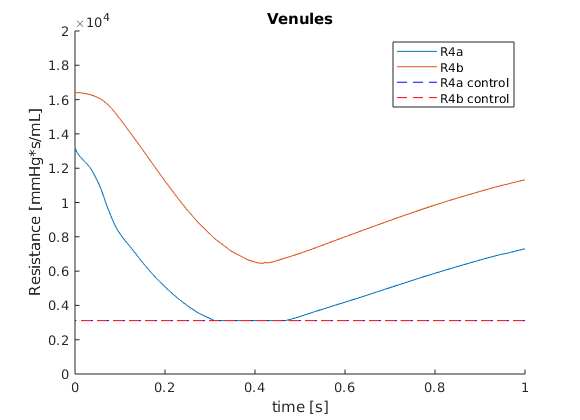
\includegraphics[width=1.0\linewidth]{Pictures/IOP30_part1/venules_30.png}
\end{subfigure}
\begin{subfigure}{.5\textwidth}
  \centering
  % include second image
  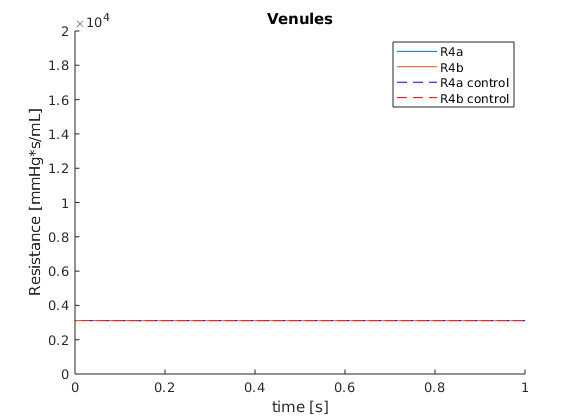
\includegraphics[width=1.0\linewidth]{Pictures/IOP15_part1/venules_15.png}
\end{subfigure}
\caption{Evoluzione della resistenza nelle venule per pazienti con $IOP = \SI{30}{\mmHg}$ a sinistra e $IOP = \SI{15}{\mmHg}$ a destra}
\label{venule1530}
\end{figure}

\begin{figure}[ht]
\begin{subfigure}{.5\textwidth}
  \centering
  % include first image
  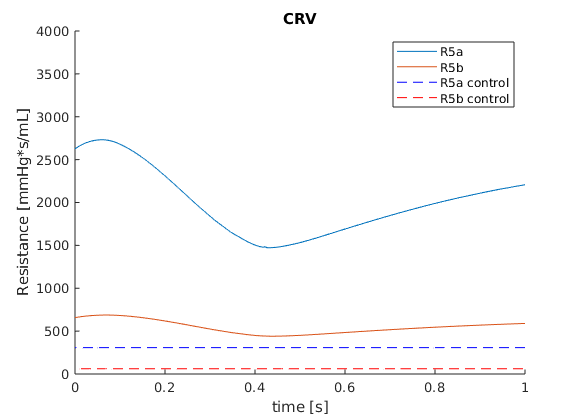
\includegraphics[width=1.0\linewidth]{Pictures/IOP30_part1/CRV_30.png}
\end{subfigure}
\begin{subfigure}{.5\textwidth}
  \centering
  % include second image
  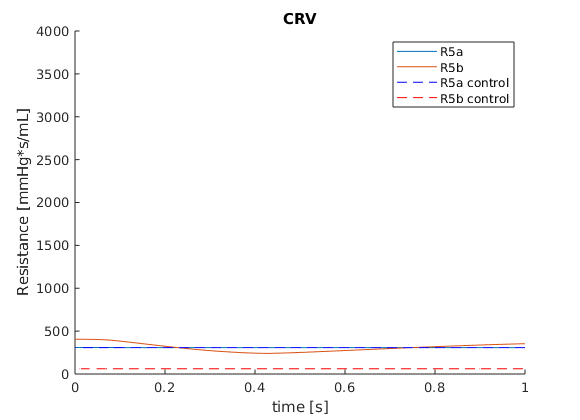
\includegraphics[width=1.0\linewidth]{Pictures/IOP15_part1/CRV_15.png}
\end{subfigure}
\caption{Evoluzione della resistenza nella CRV per pazienti con $IOP = \SI{30}{\mmHg}$ a sinistra e $IOP = \SI{15}{\mmHg}$ a destra}
\label{CRV1530}
\end{figure}

\begin{figure}[ht]
\begin{subfigure}{.5\textwidth}
  \centering
  % include first image
  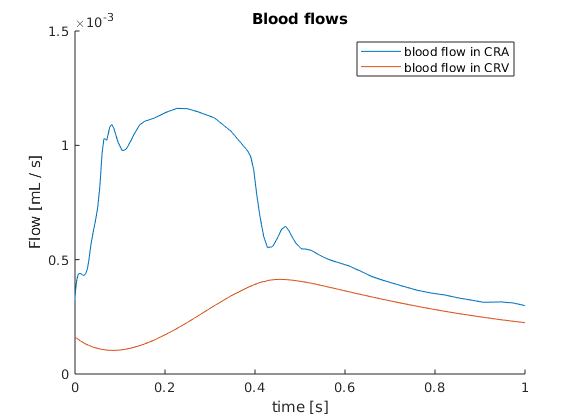
\includegraphics[width=1.0\linewidth]{Pictures/IOP30_part1/BF_30.png}
\end{subfigure}
\begin{subfigure}{.5\textwidth}
  \centering
  % include second image
  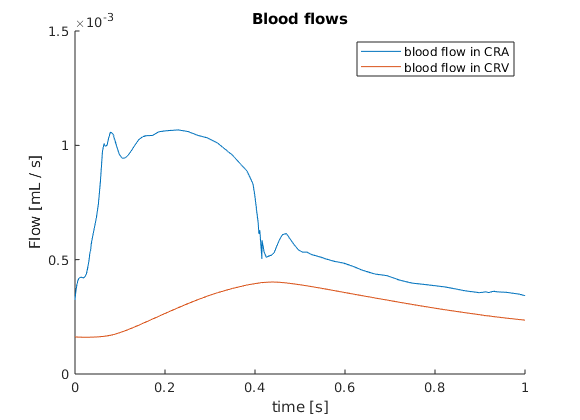
\includegraphics[width=1.0\linewidth]{Pictures/IOP15_part1/BF_15.png}
\end{subfigure}
\caption{Evoluzione della resistenza nelle venule per pazienti con $IOP = \SI{30}{\mmHg}$ a sinistra e $IOP = \SI{15}{\mmHg}$ a destra}
\label{flusso1530}
\end{figure}

Si osserva come la maggior differenza tra i due casi è dovuta allo schiacciamento delle venule e della CRV.
Il fenomeno è particolarmente evidente nella figura \ref{venule1530}: infatti per il paziente con un IOP anomalo le venule si comportano per la maggior parte del tempo come \textit{collapsible resistors} in quanto la pressione intraoculare è superiore alla pressione interna dei vasi.
Ciò non avviene per il soggetto con $IOP = \SI{15}{\mmHg}$ per cui la pressione interna delle venule riesce a compensare quella esterna e impedire lo schiacciamento.
L'effetto della maggior resistenza nelle venule si ripercuote sulla CRV, implicando una maggior caduta di pressione e quindi un valore inferiore all'interno della CRV.
Il collasso della vena è perciò dovuto sia alla maggior pressione esterna, sia all'insufficiente perssione interna.

In questo caso l'azione dell'autoregolazione nelle arteriole contrasta gli effetti dell'IOP anomalo: si può calcolare infatti che il flusso totale nei due casi nel corso della pulsazione è quasi identico ($\SI{38.4554}{\milli \liter \per \minute}$ per $IOP = \SI{15}{\mmHg}$, e $\SI{39.6301}{\milli \liter \per \minute}$ per $IOP = \SI{30}{\mmHg}$).
I risultati sono molto diversi in assenza di autoregolazione: se il flusso diminuisce leggermente nel caso di IOP normale ($\SI{36.8429}{\milli \liter \per \minute}$), esso diminuisce drasticamente a fronte di un aumento della pressione intraoculare ($\SI{32.4841}{\milli \liter \per \minute}$ per $IOP = \SI{30}{\mmHg}$).
Si conferma così l'importanza del meccanismo di autoregolazione nel mantenimento di un adeguato flusso di sangue nella microcircolazione retinica.

\begin{table}[h!]
\begin{tabular}{|c|cc|cc|}
\hline
 \textbf{autoregolazione}& \multicolumn{2}{c|}{\textbf{funzionale}} & \multicolumn{2}{c|}{\textbf{assente}} \\
 \textbf{IOP}& $\SI{15}{\mmHg}$ & $\SI{30}{\mmHg}$ & $\SI{15}{\mmHg}$ & $\SI{30}{\mmHg}$ \\
 \hline
$R_{2a}$\ $[\si{\mmHg \sec \per \milli \liter}]$ &$\num{4.56e3}$ &$\num{15.00}$ &$ \num{6.00e3}$&$ \num{6.00e3}$ \\
 Flusso totale $[\si{\milli \liter \per \minute}]$&$38.4554$&$39.6301$ &$36.8429$&$32.4841$\\
 \hline
\end{tabular}
\caption{Valori della resistenza delle arteriole e del flusso totale per diversi IOP e per autoregolazione presente o assente in un soggetto con pressione arteriosa nella norma ($\SI{80}{\mmHg}$ - $\SI{120}{\mmHg}$)}
\label{riassunto_res1}
\end{table}

\FloatBarrier
\subsection{Flusso in funzione dell'IOP}
%--------------------------------------------------------------------------------
%	CONCLUSION
%----------------------------------------------------------------------------------------
\section{Conclusione}


\addcontentsline{toc}{section}{Riferimenti bibliografici}
\bibliographystyle{unsrt}
\bibliography{sample}

%----------------------------------------------------------------------------------------


\end{document}